\chapter{Background}
\label{ch:background}

This chapter fixes the vocabulary and the notation that the rest of the
thesis uses. It defines the basic objects of a trading venue --- orders,
the limit order book, trades --- and then gives a precise description of
the two matching mechanisms compared in this thesis, the continuous double
auction (CDA) and the frequent batch auction (FBA). It closes with the
formal definition of every metric used in the empirical comparison of
\Cref{ch:results}. Why these mechanisms and these metrics matter is the
subject of \Cref{ch:foundations}; this chapter only says precisely what
they are.

\section{Basic Terminology and Notation}
\label{sec:terminology}

\subsection{Orders}

The instrument studied here is the SOL \emph{perpetual futures contract}
traded on Hyperliquid (SOL-PERP): a linear contract on the price of the
Solana token that has no expiry date, is collateralised in the USDC
stablecoin, and is kept close to the spot price of SOL by funding payments
exchanged every hour between long and short positions
\citep{hyperliquid2026docs}. One contract unit is one SOL. Prices $p$ are
quoted in US dollars per SOL (written USD throughout) and quantities $q$ in
SOL. \Cref{sec:venue} describes the venue. An \emph{order} $k$ is an
instruction to buy or sell and is described by
\begin{equation}
  k = (s_k,\; q_k,\; \pi_k,\; t_k),
\end{equation}
where $s_k \in \{\text{buy}, \text{sell}\}$ is its side, $q_k > 0$ its
quantity, $\pi_k$ its limit price and $t_k$ its submission time. A buy
order is also called a \emph{bid} and a sell order an \emph{ask}; the sets
of bids and asks in a given collection of orders are written $\mathbb{B}$
and $\mathbb{A}$.

A \emph{limit order} trades only at its limit price or better: a bid at
$\pi_k$ or lower, an ask at $\pi_k$ or higher. A \emph{market order} has no
limit and accepts any price; it is treated as a bid with no upper price
limit or an ask with no lower price limit. A \emph{cancellation} removes a
previously submitted order that has not yet been filled. An order's
\emph{time-in-force} states how long it may wait to be filled (for example
until cancelled, or immediately or never); \Cref{sec:environment} states
which of these rules the simulated engines enforce.

\subsection{The Limit Order Book}

A \emph{limit order book} is the set of limit orders that have been
submitted, not yet filled and not cancelled. These orders are said to
\emph{rest} in the book. Orders with the same limit price form a
\emph{price level}. At time $t$ the \emph{best bid} $b_t$ is the highest
resting bid price and the \emph{best ask} $a_t$ the lowest resting ask
price. Their midpoint and the quoted spread are
\begin{equation}
  \label{eq:midpoint}
  \midp = \frac{a_t + b_t}{2},
  \qquad
  \text{quoted spread}_t = a_t - b_t .
\end{equation}
The quantity resting at a price level is the \emph{depth} at that level;
the quantity at $b_t$ and $a_t$ is the depth \emph{at the best}, or at
the \emph{touch}. Relative quantities are expressed in \emph{basis points}
(bps), $1\,\text{bps} = 10^{-4}$, so that a price $p$ lies
$|p - m|/m \cdot 10^{4}$\,bps away from a reference price $m$.

\subsection{Trades, Makers and Takers}

A \emph{trade} is an exchange of quantity between one buy order and one
sell order at one price. When an arriving order is matched against a
resting order, the resting order is the \emph{maker} (it supplied
liquidity) and the arriving order the \emph{taker} or \emph{aggressor} (it
demanded liquidity). A trade is indexed like an order: trade $k$ has price
$p_k$, quantity $q_k$ and time $t_k$, and whether $k$ denotes an order or a
trade is always clear from context. The direction of trade $k$ is
$\varepsilon_k = +1$ if the aggressor was a buyer and $\varepsilon_k = -1$
if it was a seller. The signed quantity $\varepsilon_k q_k$, summed over a
set of trades, is their net \emph{order flow}: positive when buying
pressure dominates. A participant who quotes on both sides of the book to
earn the spread is a \emph{market maker} or \emph{liquidity provider}.

\Cref{tab:notation} collects every symbol used in the thesis, grouped by
topic, with the section in which each is defined.

\begingroup
\small
\renewcommand{\arraystretch}{1.15}
\begin{longtable}{@{}p{3.3cm} p{10.4cm} p{2.0cm}@{}}
\caption[Notation]{Notation used throughout the thesis.}
\label{tab:notation}\\
\toprule
\textbf{Symbol} & \textbf{Meaning} & \textbf{Defined in}\\
\midrule
\endfirsthead
\multicolumn{3}{@{}l}{\emph{\Cref{tab:notation}, continued}}\\
\toprule
\textbf{Symbol} & \textbf{Meaning} & \textbf{Defined in}\\
\midrule
\endhead
\bottomrule
\endfoot
\multicolumn{3}{@{}l}{\emph{Orders, book and trades}}\\
$p,\ q$ & a price (USD per SOL) and a quantity (SOL) & \S\ref{sec:terminology}\\
$k$ & index of an order, or of a trade & \S\ref{sec:terminology}\\
$s_k, q_k, \pi_k, t_k$ & side, quantity, limit price and submission time of order $k$ & \S\ref{sec:terminology}\\
$j$ & a resting order that an arriving order trades against (CDA) & \S\ref{sec:cdaformal}\\
$\mathbb{B}, \mathbb{A}$ & sets of bids (buy orders) and asks (sell orders) of a batch or a book & \S\ref{sec:terminology}\\
$b_t, a_t$ & best bid and best ask of the CDA book at time $t$ & \S\ref{sec:terminology}\\
$\midp$ & midpoint $(a_t + b_t)/2$ of the CDA book at time $t$ & \eqref{eq:midpoint}\\
$m$ & a reference price against which a distance in bps is measured & \S\ref{sec:terminology}\\
$p_k, q_k, t_k$ & price, quantity and time of trade $k$ & \S\ref{sec:terminology}\\
$\varepsilon_k$ & direction of trade $k$: $+1$ buyer-initiated, $-1$ seller-initiated & \S\ref{sec:terminology}\\
\midrule
\multicolumn{3}{@{}l}{\emph{Batch clearing}}\\
$\tau$ & batch interval of the FBA; also the width of a measurement bucket ($\tau = 1$\,s in the run) & \S\ref{sec:fbanotation}\\
$\mathbf{1}\{\cdot\}$ & indicator function: $1$ if the condition holds, $0$ otherwise & \eqref{eq:demandsupply}\\
$D(p), S(p)$ & cumulative demand and supply of a batch at price $p$ & \eqref{eq:demandsupply}\\
$V(p)$ & executable volume $\min\{D(p), S(p)\}$ at price $p$ & \S\ref{sec:fbanotation}\\
$\mathcal{P}^{*}$ & set of volume-maximising prices & \S\ref{sec:fbanotation}\\
$\underline{p}, \overline{p}$ & lowest and highest price in $\mathcal{P}^{*}$ & \S\ref{sec:fbanotation}\\
$V^{*}$ & maximal executable volume of a batch & \S\ref{sec:fbanotation}\\
$\sigma$ & tie-break rule selecting one price from $\mathcal{P}^{*}$ & \eqref{eq:clearing}\\
$\clr$ & clearing price of a batch, $\clr = \sigma(\mathcal{P}^{*})$ & \eqref{eq:clearing}\\
$p_{\mathrm{prev}}$ & clearing price of the previous batch that traded (tie-break step 3) & \S\ref{sec:fbanotation}\\
$x_k$ & quantity of order $k$ executed in a batch & \S\ref{sec:fbanotation}\\
\midrule
\multicolumn{3}{@{}l}{\emph{Surplus}}\\
$W^{\mathbb{B}}(p), W^{\mathbb{A}}(p)$ & buyer and seller surplus (price improvement against own limits) of a batch at price $p$ & \eqref{eq:surplus}\\
$W$ & total surplus of a batch, $W = W^{\mathbb{B}}(\clr) + W^{\mathbb{A}}(\clr)$; independent of the price chosen in $\mathcal{P}^{*}$ & \eqref{eq:surplus}, \eqref{lem:invariance}\\
\midrule
\multicolumn{3}{@{}l}{\emph{Measurement grid}}\\
$t_0$ & timestamp of the first record of the run & \eqref{eq:bucket}\\
$\mathrm{bucket}(t)$ & the one-second bucket containing time $t$ & \eqref{eq:bucket}\\
$e$ & engine, $e \in \{\mathrm{CDA}, \mathrm{FBA}\}$ & \S\ref{sec:measurement}\\
$M^{e}_t$ & value of metric $M$ for engine $e$ in bucket $t$ & \S\ref{sec:measurement}\\
$d_t$ & paired difference $M^{\mathrm{FBA}}_t - M^{\mathrm{CDA}}_t$ & \S\ref{sec:measurement}\\
$n$ & number of buckets (or days) with a paired value & \S\ref{sec:experiments}\\
\midrule
\multicolumn{3}{@{}l}{\emph{Metrics}}\\
$h$ & distance threshold of depth within $h$ bps, $h \in \{10, 50, 100\}$ & \S\ref{sec:metrics21}\\
$m_k$ & pre-trade reference price of trade $k$ & \S\ref{sec:metrics21}\\
$\Delta$ & markout horizon, $\Delta \in \{1, 5, 30\}$\,s & \S\ref{sec:metrics21}\\
$m_{k+\Delta}$ & first reference price at or after $t_k + \Delta$ & \S\ref{sec:metrics21}\\
$S^{\mathrm{eff}}_k$ & effective spread of trade $k$ & \eqref{eq:effspread}\\
$S^{\mathrm{real}}_k(\Delta)$ & realized spread of trade $k$ at horizon $\Delta$ & \eqref{eq:realspread}\\
$\mathrm{PI}_k(\Delta)$ & price impact of trade $k$ at horizon $\Delta$ & \eqref{eq:priceimpact}\\
$r_i$ & $i$-th consecutive return of the reference price within a bucket & \S\ref{sec:formularq22}\\
$\mathcal{T}$ & set of buckets in which both engines traded & \S\ref{sec:formularq22}\\
$\mathrm{VWAP}^{e}_t$ & volume-weighted average price of engine $e$ in bucket $t$ & \S\ref{sec:formularq22}\\
$r^{e}_i$ & log return of $\mathrm{VWAP}^{e}$ between consecutive buckets of $\mathcal{T}$ & \eqref{eq:matchedvol}\\
$\mathrm{vol}^{e}_{\text{day}}$ & matched-timestamp volatility of engine $e$ on one day & \eqref{eq:matchedvol}\\
$\lambda$ & Kyle's lambda, price change per unit of net order flow & \S\ref{sec:formularq22}\\
$f_i$ & venue net taker flow in second $i$ (1{,}000 SOL), the regressor of Kyle's lambda & \eqref{eq:kylef}\\
$y^{e}_i(h)$ & price change (bps) of engine $e$ from second $i-1$ to $i+h$ & \eqref{eq:kyley}\\
$\lambda^{e}(h), u^{e}_i$ & Kyle's lambda of engine $e$ at horizon $h$, and the regression residual & \eqref{eq:kylereg}\\
$\theta(h), v_i$ & difference $\lambda^{\mathrm{FBA}}(h) - \lambda^{\mathrm{CDA}}(h)$, and its regression residual & \eqref{eq:kylediff}\\
$m_{\mathrm{pre}}, m_{\mathrm{post}}$ & CDA midpoint before a sweep and 5\,s after it (per-sweep CDA lambda) & \S\ref{sec:formularq22}\\
$\mu$ & prior expected value of the asset in the model of \citet{kyle1985continuous} & \S\ref{sec:adverse}\\
\midrule
\multicolumn{3}{@{}l}{\emph{Design analysis}}\\
$\delta$ & difference in message latency between two participants & \S\ref{sec:interval}\\
$\tau_{\min}, \tau_{\max}$ & bounds of a randomised closing time & \S\ref{sec:interval}\\
$i$ & a participant (in sums: an observation index) & \S\ref{sec:priceimprovement}\\
$\ell_i$ & message latency of participant $i$ & \eqref{prop:latency}\\
$\kappa$ & share of the marginal volume allocated pro rata in a hybrid rationing rule & \S\ref{sec:rationing}\\
\end{longtable}
\endgroup

\section{The Continuous Double Auction}
\label{sec:cdaformal}

The CDA processes orders one at a time, in the order the venue receives
them, against a limit order book. Resting orders are ranked by
\emph{price-time priority}: a better price first, and among orders at the
same price, the earlier one first. When a buy order $k$ arrives, it is
matched as follows (a sell order is symmetric, with bids in place of
asks):
\begin{enumerate}
  \item While $k$ has quantity left and the book holds an ask with
  $a_t \le \pi_k$ (always, for a market order), $k$ trades against the
  first-ranked order $j$ at the best ask. The trade price is the
  \emph{resting} order's price, $p = a_t$, and the trade quantity is the
  smaller of the two orders' remaining quantities; both are reduced by it,
  and a fully filled resting order leaves the book.
  \item Any quantity of a limit order that is left when no further ask
  crosses rests in the book at $\pi_k$, behind the orders already resting
  at that price. The unfilled remainder of a market order does not rest.
\end{enumerate}
Three properties of this rule matter for the comparison. Execution is
immediate: an order that can trade does so the instant it arrives. A
single order that sweeps several price levels trades at several prices.
And the maker--taker distinction is defined by arrival order, so every
CDA trade has a known aggressor and direction $\varepsilon_k$.

\section{The Frequent Batch Auction}
\label{sec:fbanotation}

A frequent batch auction collects orders over a half-open window $[0,\tau)$
of length $\tau$ and, at the end of the window, considers all of them
together instead of one at a time. Let $\mathbb{B}$ and $\mathbb{A}$
denote the sets of bids and asks in the batch. A market bid is treated as
having no upper price limit and a market ask as having no lower price
limit, so it never falls out of either schedule below on grounds of
price.

\subsection{Demand and Supply}

The batch is cleared by lining up how much would be bought against how much
would be sold at every possible price, and finding where the two balance.
For any price $p$, the bid side gives the cumulative \emph{demand} at that
price and the ask side gives the cumulative \emph{supply}.
Demand is the quantity buyers are willing to take at $p$ or less, so it can
only fall as $p$ rises: a bid counts toward it once its limit price is at
least $p$, and drops out as soon as $p$ climbs past that limit. Supply is
the mirror image: the quantity sellers are willing to give up at $p$ or
more, which can only rise as $p$ rises, since an ask counts once its limit
price is at most $p$. Written out, with the market-order convention above,
\begin{equation}
  \label{eq:demandsupply}
  D(p) = \sum_{k \in \mathbb{B}} q_k \mathbf{1}\{\pi_k \ge p\},
  \qquad
  S(p) = \sum_{k \in \mathbb{A}} q_k \mathbf{1}\{\pi_k \le p\}.
\end{equation}
Plotted against price, $D$ and $S$ are \emph{step} curves rather than
smooth ones, because each order adds its whole quantity at once, the
moment its limit price is reached, rather than a little at a time: $D$
steps down as price rises, $S$ steps up. \Cref{fig:fbaschedule} shows
exactly this picture for a small worked example. At any price $p$, only
the smaller of the two sides can actually trade, so the volume executable
at that price is
\begin{equation}
  V(p) = \min\{D(p), S(p)\}.
\end{equation}

\begin{figure}[htbp]
\centering
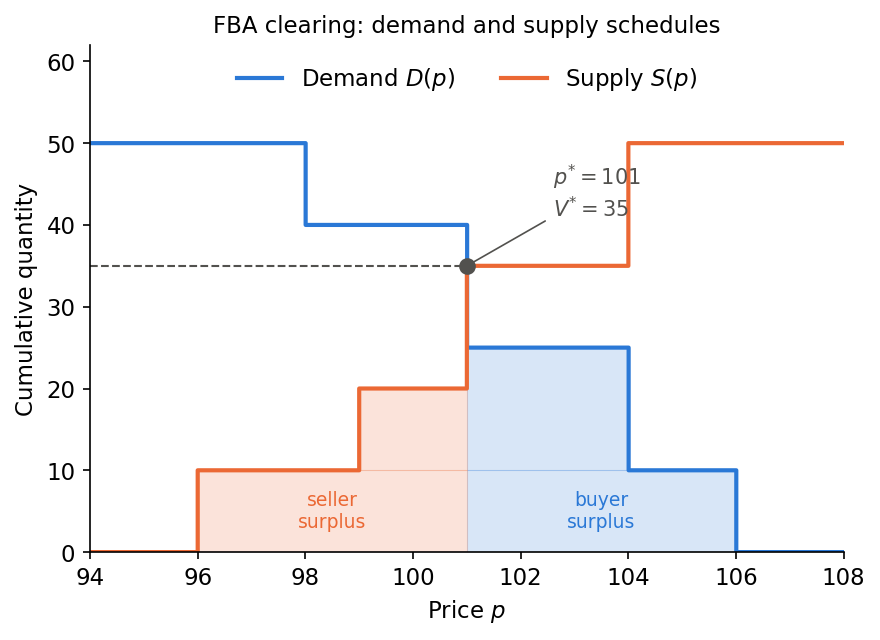
\includegraphics[width=0.72\textwidth]{figures/fig_fba_schedule.png}
\caption[FBA clearing as a supply/demand diagram]{The FBA clearing
mechanism drawn as a classical demand/supply diagram: $D(p)$ and $S(p)$
as step functions of price. Reading it: pick any price on the horizontal
axis; the height of the demand step there is how much would be bought at
that price or cheaper, the height of the supply step is how much would be
sold at that price or dearer. The two curves cross at the clearing price
$\clr = 101$, where the executable volume $V(p)$ is largest
($V^{*} = 35$). Drawn from a small illustrative batch of eight orders,
four buys (limits 106, 104, 101, 98) and four sells (limits 96, 99, 101,
104), chosen because it clears without a tie and so needs no tie-break
cascade (below). At $\clr$ demand exceeds supply by 5, so the buy order
at 101 is only partly filled. The shaded areas are the buyers' surplus
(right of $\clr$, under $D$) and the sellers' surplus (left of $\clr$,
under $S$), built from one rectangle per order that trades at a better
price than its limit. A real batch from the simulated month has dozens
of orders and does not render legibly at this scale.}
\label{fig:fbaschedule}
\end{figure}

\subsection{Finding the Clearing Price}

The two curves do not have to cross at one exact price: they can run side
by side, both holding the same height, across several price ticks at
once, which happens often when the book is thin. Every price in that
stretch executes the same maximum volume, so volume by itself cannot say
which one is actually used. The clearing rule therefore works in two
stages. First, it finds every price that reaches the greatest executable
volume, the volume-maximising set
\begin{equation}
  \mathcal{P}^{*} = \argmax_{p \in \mathbb{R}_{+}} V(p),
  \qquad V^{*} = \max_{p} V(p),
\end{equation}
which, since $D$ is non-increasing and $S$ is non-decreasing, is a single
closed interval $[\underline{p}, \overline{p}]$ whenever the book crosses
at all ($V^{*} > 0$). When that interval holds more than one price, a
second, tie-breaking stage is needed to pick exactly one of them:
\begin{equation}
  \label{eq:clearing}
  \clr = \sigma\bigl(\mathcal{P}^{*}\bigr) \in \mathcal{P}^{*}.
\end{equation}
Real auctions resolve this indeterminacy with a fixed cascade of
tie-breaking steps, applied in order until one price remains
\citep{haynes2020precedence}, and the engine used in this thesis follows
exactly this cascade (\Cref{app:config}):
\begin{enumerate}
  \item choose the price (or prices) that maximise $V(p)$ --- this is
  $\mathcal{P}^{*}$ itself;
  \item if $\mathcal{P}^{*}$ is not a singleton, choose the price that
  minimises the residual imbalance $|D(p) - S(p)|$;
  \item if still tied, choose the price closest to the auction's own
  previous clearing price $p_{\mathrm{prev}}$;
  \item if still tied, choose the lowest such price.
\end{enumerate}

\subsection{Allocation, Rationing and the Residual}

Let $x_k \ge 0$ denote the executed quantity of order $k$ under a
volume-maximising allocation, so that $\sum_{k \in \mathbb{B}} x_k =
\sum_{k \in \mathbb{A}} x_k = V^{*}$. Every trade of the batch is at the
single price $\clr$. At $\clr$ the two sides are usually not equal,
$D(\clr) \ne S(\clr)$, so the orders on the longer side cannot all be
filled and a \emph{rationing rule} decides which are. The engine used here
ranks the eligible orders of each side by \emph{price-time priority within
the batch}: market orders first, then the better limit price, then the
earlier submission, and fills them in that order until the shorter side
is used up (\Cref{sec:rationing} discusses the alternatives). The volume
left unmatched, $|D(\clr) - S(\clr)|$ on the longer side together with
every order that was not eligible at $\clr$, is the \emph{residual}; in
this thesis it rolls over into the next batch with its limit price and
submission time unchanged.

\subsection{Price Improvement and Surplus}

Uniform pricing gives every executed order a price at least as good as
the one it asked for, and every inframarginal order a strictly better
one; \Cref{fig:fbaschedule} shows exactly how much better. A buyer
with limit price $\pi_k$ above $\clr$ does not pay $\pi_k$; the whole
batch pays $\clr$, so this order keeps the gap $\pi_k - \clr$ for every
unit it trades. In \Cref{fig:fbaschedule} each such order is one shaded
rectangle: its width is how far that order's limit sits above the
clearing price, its height is how much of it trades, and its area is
what that order gains by not having to pay what it was willing to.
Sellers gain the mirror amount, $\clr - \pi_k$, the gap between the
clearing price and their own limit. Summed over every executed order,
these gaps are the familiar consumer- and producer-surplus areas of a
supply/demand diagram, read off a single discrete batch instead of a
continuous market. With price on the horizontal axis, as in
\Cref{fig:fbaschedule}, the buyers' share is the area to the right of
$\clr$ under the demand curve, and the sellers' share is the area to the
left of $\clr$ under the supply curve.

Formally, each side's surplus at a candidate price $p$ is
\begin{equation}
  \label{eq:surplus}
  W^{\mathbb{B}}(p) = \sum_{k \in \mathbb{B}} (\pi_k - p)\, x_k,
  \qquad
  W^{\mathbb{A}}(p) = \sum_{k \in \mathbb{A}} (p - \pi_k)\, x_k,
\end{equation}
and total surplus at the batch's own clearing price is $W =
W^{\mathbb{B}}(\clr) + W^{\mathbb{A}}(\clr)$. Every
term in both sums is non-negative for an executed order --- a buy only
has $x_k>0$ if $\pi_k \ge \clr$, and a sell only if $\pi_k \le \clr$, so
no order ever executes at a loss relative to its own limit. This is what
\Cref{ch:results} measures as \emph{trader surplus}. The worked example
also previews a point \Cref{sec:priceimprovement} returns to in full: the
two sides need not split $W$ evenly. Here the buyers gain
$5 \times 10 + 3 \times 15 = 95$ and the sellers
$5 \times 10 + 2 \times 10 = 70$, while the buy and the sell with limit
101 trade exactly at their limit and gain nothing. In this example
$\mathcal{P}^{*}$ holds the single price $101$, so the split is pinned
down; when $\mathcal{P}^{*}$ holds
several prices, choosing a different one would split $W$ differently
without changing who trades or how much.

\subsection{What Differs from the CDA}
\label{sec:fbavscda}

Set against \Cref{sec:cdaformal}, the FBA changes three things. Orders
wait up to $\tau$ for their first chance to trade, instead of trading on
arrival, and longer if they are rolled over.
All trades of a batch share one price $\clr$, instead of each trading at
the resting order's price. And because the orders of a batch trade
simultaneously, no order crosses another's quote: there is no maker and
no taker, and a trade has no observable direction $\varepsilon_k$. This
point is one reason several metrics below need an adaptation for the
FBA. The other reason is less obvious but matters just as much: the FBA
has no order book that could be observed in the way the CDA's can.

\paragraph{Why the FBA's unmatched orders are not an order book.} At
first sight the FBA seems to offer a ready-made substitute for the CDA's
book. At any moment it holds a set of orders that have not traded yet,
each with a side, a quantity and a limit price. Sorted by price, this set
would give a best bid, a best ask, depth at every level and a book
imbalance, and every book-based statistic could then be computed exactly
as for the CDA. This does not work, because the two sets are produced by
different processes and therefore mean different things.

A CDA book is what remains \emph{after} matching. Every order that can
trade does so the instant it arrives (\Cref{sec:cdaformal}), so an order
sits in the book only because no opposite order has been willing to trade
with it. The book is therefore never crossed ($b_t < a_t$ at all times),
and its depth is liquidity that is actually available: a new order can
trade against it immediately, at the prices shown.

The FBA's pending orders are what is waiting \emph{for} matching: the
residual of the last batch plus everything submitted since. None of
these orders has yet been matched against any other, which has three
consequences.
\begin{itemize}
  \item \textbf{The set holds orders a CDA book never would.} A buy
  priced above a waiting sell would have traded on arrival in the CDA; in
  the FBA both simply wait for the close. Whenever a batch is going to
  trade, its pending set is crossed, with the best buy at or above the
  best sell. Its ``quoted spread'' is then zero or negative, and its depth
  includes quantity that is about to disappear.
  \item \textbf{Its content depends on when it is read.} Just after a
  clear it holds only the residual; just before the next clear it holds
  the residual plus a full interval of new orders. A CDA book has no such
  cycle.
  \item \textbf{Nobody can trade against it at the prices shown.} A
  pending order offers to trade only at the next clearing price, and only
  if that batch's demand and supply reach its limit. It is not standing
  liquidity at its own limit price in the moment it is observed.
\end{itemize}
Statistics computed on the pending set as if it were a book would measure
the batching delay rather than the liquidity of the market. For the same
reason, Kyle's lambda is not estimated from the pending set: both engines
are measured against one common measure of order flow, the venue's own
net taker flow (\Cref{sec:formularq22}).

\paragraph{When the FBA is read: before the close, after the clear, or at
the CDA's times.} Any book-like FBA statistic must be read at some point
in the batch cycle, and that choice decides which way the comparison is
biased.
\begin{itemize}
  \item \textbf{Just before the close} the pending set is at its fullest:
  it holds the whole interval's orders, including those that are about to
  execute. Depth read here is overstated, so the bias \emph{favours} the
  FBA. Both depth measures in this thesis are read at this point
  (\Cref{sec:metrics21}). The FBA still comes out slightly thinner, so
  that finding holds with margin.
  \item \textbf{Just after the clear} the residual is, like a CDA book,
  no longer crossed, because everything that could trade at $\clr$ has
  traded. But this is the thinnest moment of the cycle. The clear has
  just removed exactly the orders closest to $\clr$, and the next
  interval's orders have not arrived yet, so the residual is often
  one-sided near $\clr$. A spread or depth read here is biased
  \emph{against} the FBA. The FBA quoted spread is read at this point,
  which is one reason it is treated as weaker evidence
  (\Cref{sec:limitscomparable}).
  \item \textbf{At the CDA's snapshot times.} One could instead read the
  pending set at the same instants as the CDA's book snapshots, so that
  both engines are observed ``at the same time''. The same clock time
  does not make the two sets the same kind of object. At any instant
  inside a batch, the pending set is the residual plus whatever has
  arrived so far. It is still unmatched and possibly crossed, and its
  content depends on how far into the batch the snapshot falls.
  Averaging such readings over the interval only mixes the two biases
  above, in proportions set by when orders happen to arrive.
\end{itemize}
The sampling also differs. A CDA bucket value is the mean of many book
snapshots spread across the second (\Cref{sec:metrics21}), which
describes the typical state of the book. An FBA value is a single reading
per batch, taken at one end of the cycle.

For these reasons the comparison rests mainly on \emph{trades}. A trade
exists only once matching is complete, in both mechanisms: in the CDA
at the instant two orders cross, and in the FBA at the instant the batch
clears. Executed volume, effective and realized spread, price impact and
trader surplus therefore compare like with like, whenever they are read.
The book-like FBA metrics are kept, but each is read at a stated point in
the cycle, and its direction of bias is taken into account when the
results are interpreted. \Cref{app:comparability} sets out the argument
in more detail.

\section{Measurement Framework}
\label{sec:measurement}

Both engines are measured on one common time grid. Every observation is
assigned to a fixed-width time \emph{bucket},
\begin{equation}
  \label{eq:bucket}
  \mathrm{bucket}(t) = t_0 + \left\lfloor \frac{t - t_0}{\tau} \right\rfloor \tau,
\end{equation}
where $t_0$ is the timestamp of the first record of the run and the
width equals the batch interval, $\tau = 1$\,second throughout this
thesis. Every metric below is computed once per bucket and per engine, so
each bucket yields one CDA value and one FBA value from the same order
flow. Buckets are contiguous: a bucket with no qualifying observation
still exists, with the metric marked missing. A missing value (``no
qualifying observation in this bucket'') and a value of zero (``there were
observations and the value is zero'') are kept distinct.

For a metric $M$ computable on both engines, the comparison is the
\emph{paired difference} $d_t = M^{\mathrm{FBA}}_t - M^{\mathrm{CDA}}_t$
over the buckets in which both values exist; \Cref{sec:experiments}
describes how its standard error is estimated. A metric that exists for
only one engine is reported descriptively.

\section{Metrics}
\label{sec:metricdefs}

Each metric below is tagged with its \emph{scope}: \textbf{U} (computed for
both engines) or \textbf{F} (FBA only). The metrics are grouped by
the part of RQ2 (\Cref{sec:rqs}) they answer. \Cref{tab:metrics} gives an
overview; \Cref{ch:foundations} explains why each is used.

\begin{table}[htbp]
\centering
\caption[Overview of the metrics]{Overview of the metrics, by research
question. Scope: U both engines, F FBA only.}
\label{tab:metrics}
\small
\begin{tabularx}{\textwidth}{@{}l l L c@{}}
\toprule
\textbf{RQ} & \textbf{Metric} & \textbf{What it measures} & \textbf{Scope}\\
\midrule
2.1 & Quoted spread & cost of crossing the book now & U\\
    & Depth at best / within $h$ bps & quantity available near the price & U\\
    & Effective spread & cost an actual trade paid & U\\
    & Realized spread & part of that cost the maker keeps & U\\
    & Price impact & part lost to informed traders & U\\
    & Amihud illiquidity & price move per dollar traded & U\\
\midrule
2.2 & Matched-timestamp volatility & price variability on a common grid & U\\
    & Intra-interval dispersion & price variation within one second & U\\
    & Kyle's lambda & price move per unit of the venue's net order flow & U\\
\midrule
2.3 & Executed volume, trade count & how much trades & U\\
    & Time to execution & how long orders wait & U\\
    & Trader surplus & price improvement against the limit & U\\
    & Boundary concentration & arrivals near the batch close & F\\
    & Unexecuted residual share & imbalance left at $\clr$ & F\\
\midrule
--- & Throughput, clearing latency & computing speed (control) & U\\
\bottomrule
\end{tabularx}
\end{table}

\subsection{Liquidity and Transaction Costs (RQ2.1)}
\label{sec:metrics21}

\paragraph{Quoted spread (U).} For the CDA, every book snapshot in the
bucket with both sides present contributes $(a_t - b_t)/\midp \cdot
10^{4}$\,bps, and the bucket value is the mean over snapshots. The FBA
has no book while a batch accumulates; its analogue is the gap between the
best unfilled sell and the best unfilled buy among the orders left after
a clear (including those rolled over from earlier batches), relative to
$\clr$ and in bps, averaged over the batches in which both exist.

\paragraph{Depth at best (U).} For the CDA, the mean over snapshots of
(best-bid size $+$ best-ask size)$/2$, the touch only. For the FBA, the
mean over batches of $(D(\clr) + S(\clr))/2$, the quantity eligible to
trade at the clearing price.

\paragraph{Depth within $h$ bps (U), $h \in \{10, 50, 100\}$.} The
quantity of all orders priced within $h$\,bps of a reference price, half
the sum of both sides, cumulative across thresholds. The orders counted
are those in the book (CDA, reference $\midp$) or pending in the batch
just before it clears (FBA, rolled-over orders included, reference
$\clr$).

\paragraph{Effective, realized spread and price impact (U).} Let trade
$k$ have price $p_k$, direction $\varepsilon_k$, pre-trade reference price $m_k$
and, a markout horizon $\Delta$ later, reference price $m_{k+\Delta}$.
In proportional form \citep{hasbrouck1993assessing,hendershott2011algorithmic},
\begin{align}
  S^{\mathrm{eff}}_k &= \frac{2 \varepsilon_k (p_k - m_k)}{m_k},
    \label{eq:effspread}\\[3pt]
  S^{\mathrm{real}}_k(\Delta) &= \frac{2 \varepsilon_k (p_k - m_{k+\Delta})}{m_k},
    \label{eq:realspread}\\[3pt]
  \mathrm{PI}_k(\Delta) &= \frac{2 \varepsilon_k (m_{k+\Delta} - m_k)}{m_k},
    \label{eq:priceimpact}
\end{align}
each in bps after multiplying by $10^{4}$, so that $S^{\mathrm{eff}}_k =
S^{\mathrm{real}}_k(\Delta) + \mathrm{PI}_k(\Delta)$ trade by trade and in
any quantity-weighted aggregate. The bucket value is the
quantity-weighted mean over the bucket's trades, for $\Delta \in
\{1, 5, 30\}$\,s. For the CDA, $m_k$ is the book midpoint just before the
trade (the best price of the one side present, if the other side is
empty) and $m_{k+\Delta}$ the first midpoint at or after $t_k + \Delta$.
The FBA needs two adaptations. Its reference price $m_k$ is the clearing
price of the last earlier batch that traded, $p_{\mathrm{prev}}$, since
there is no midpoint while a batch accumulates, and $m_{k+\Delta}$ is the
first FBA clearing price at or after $t_k + \Delta$. And its trades have no direction $\varepsilon_k$
(\Cref{sec:fbanotation}), so the simulator records only the unsigned
deviation $2|p_k - m_k|/m_k$.

\paragraph{Signing the FBA side.} Before the FBA values are compared, each
bucket in which both engines traded is given a direction by a zero-tick
rule \citep{leeready1991} applied to the \emph{CDA's} prices: taking these
buckets in time order, a bucket's FBA trades are labelled buys if the CDA's
VWAP rose from the previous such bucket, sells if it fell, and inherit the
last nonzero tick if it is unchanged. The reported
FBA effective and realized spread are this sign times the unsigned
values, and the FBA price impact is the signed effective spread minus the
signed realized spread. Signing with the FBA's own price history instead
would be circular, because that history is $m_k$ itself, so the sign
would only undo the deviation's own sign. The rule is an estimate, not
an observed direction; \Cref{sec:limitssign} discusses what it can and cannot
recover.

\paragraph{Amihud illiquidity (U).} With $\mathrm{close}$ the last
reference price observed in a bucket (carried forward across empty
buckets) and $\mathrm{ret} = (\mathrm{close} -
\mathrm{prev\_close})/\mathrm{prev\_close}$,
\begin{equation}
  \label{eq:amihud}
  \mathrm{Amihud} = \frac{|\mathrm{ret}|}{\text{dollar volume}} \cdot 10^{6}
\end{equation}
for every bucket that traded a nonzero volume \citep{amihud2002illiquidity};
it is missing otherwise, so a price move on zero volume is not recorded as
infinite illiquidity.

\subsection{Price Discovery and Market Quality (RQ2.2)}
\label{sec:formularq22}

\paragraph{Realized volatility (U).} Within a bucket, the root sum of
squared consecutive returns of the reference price,
$\sqrt{\sum_i r_i^2}$. It needs at least two prices in one bucket, which
the FBA, clearing at most once per second, almost never has; it is
therefore not used for the comparison, and is replaced by the next metric.

\paragraph{Matched-timestamp volatility (U).} Let $\mathcal{T}$ be the set
of buckets in which both engines traded, with $\mathrm{VWAP}^{e}_t$ the
volume-weighted average price of engine $e$ in bucket $t$. Over
consecutive $t_i, t_{i+1} \in \mathcal{T}$ the two engines' log returns
$r^{e}_i = \ln(\mathrm{VWAP}^{e}_{t_{i+1}} / \mathrm{VWAP}^{e}_{t_i})$ are
computed over the \emph{same} instants for both. They are grouped by the
calendar day of $t_{i+1}$ and summarised as
\begin{equation}
  \label{eq:matchedvol}
  \mathrm{vol}^{e}_{\text{day}} = \sqrt{\operatorname{mean}_i\, (r^{e}_i)^2}
  \cdot 10^{4}\ \text{bps},
\end{equation}
a root \emph{mean} square, so that a busier day is not mistaken for a more
volatile one. A day with fewer than 5 matched returns is excluded for both
engines. Because $\mathcal{T}$ needs a trade on both sides, the measure
compares the engines on common ground; it is not a whole-month volatility
estimate for either.

\paragraph{Intra-interval price dispersion (U).} The coefficient of
variation of the trade prices within a bucket,
$\operatorname{std}(\{p_k\}) / \operatorname{mean}(\{p_k\}) \cdot
10^{4}$\,bps (population standard deviation). It is zero for the FBA by
construction whenever the bucket holds a single batch clear, since every
trade of a batch is at $\clr$.

\paragraph{Kyle's lambda (U).} Kyle's lambda measures how far the price
moves per unit of net order flow \citep{kyle1985continuous}. It is
estimated as the slope of a regression of price change $y$ on net signed
flow $f$; the regressor, the response and the regression itself are set
out in turn below.

The FBA poses a problem for the regressor $f$. Net order flow is normally
read from the trades themselves, as buyer-initiated minus
seller-initiated quantity, $\sum_k \varepsilon_k q_k$
(\Cref{sec:terminology}). In the CDA every trade has an aggressor, so
this is possible. In the FBA it is not: all orders of a batch trade at
once, no trade has an aggressor, and $\varepsilon_k$ does not exist
(\Cref{sec:fbavscda}). The FBA therefore has no net order flow of its
own to put on the right-hand side of the regression.

The solution is to measure the flow \emph{outside} both engines and use
that one series for both. The raw Hyperliquid records have no aggressor
field, but they allow the aggressor to be identified. Every fill on the
real venue writes a record with status \emph{filled}, the order's side
and its remaining size, and each record carries the time elapsed since
the order was submitted (\texttt{timestampDiff}, in milliseconds). A
fill recorded at the order's own submission time, with an elapsed time
of zero, means the order traded on arrival: it took liquidity and was
the taker. A fill recorded later belongs to an order that had been
resting, a maker. The filled quantity is the drop in the order's
remaining size. Summing the taker fills by side gives the venue's net
taker flow in each second $i$,
\begin{equation}
  \label{eq:kylef}
  f_i = \frac{\text{taker buy quantity}_i - \text{taker sell quantity}_i}{1{,}000\ \text{SOL}},
\end{equation}
positive when buyers were the aggressors on balance. Three properties
make it the right regressor. It is identical for both engines, because
both replay the same orders in the same second. Its direction comes from
the venue's own fill records, not from a price-based guess such as the
tick rule used for the FBA spreads; the only error left is a maker hit
within the first millisecond after it was posted, which the record's
millisecond resolution would count as a taker. And it comes from neither of the two engines
being compared: the simulator never reads these records. Using the
CDA's own executed flow instead would have measured the FBA against a
quantity produced by its competitor. The CDA's simulated volume follows
the venue's closely over time, but at about twice its level, because the
replay does not enforce all of the venue's rules
(\Cref{sec:testfidelity}); the venue's own record avoids that error too.

With $f_i$ fixed, each engine is regressed on it separately. The response
is that engine's own price change,
\begin{equation}
  \label{eq:kyley}
  y^{e}_i(h) = \frac{P^{e}_{i+h} - P^{e}_{i-1}}{P^{e}_{i-1}} \cdot 10^{4},
  \qquad h \in \{0, 5\}\,\text{s},
\end{equation}
where $P^{e}_i$ is engine $e$'s VWAP in second $i$, carried forward over
seconds in which it did not trade. Lambda is then the slope of a linear
regression of this price change on the flow, estimated separately for
each engine $e$ and each horizon $h$:
\begin{equation}
  \label{eq:kylereg}
  y^{e}_i(h) = \lambda^{e}(h)\, f_i + u^{e}_i,
  \qquad
  \hat{\lambda}^{e}(h) = \frac{\sum_i f_i\, y^{e}_i(h)}{\sum_i f_i^{2}},
\end{equation}
where $u^{e}_i$ is the part of the price change not explained by the
flow. The regression is estimated by ordinary least squares
\emph{without an intercept}: Kyle's price rule $p = \mu + \lambda f$
(\Cref{sec:adverse}) says that with no net flow the price should not
move, so the line is forced through the origin, and the
estimator is the ratio given in \eqref{eq:kylereg}. The question each
slope answers is the same for both engines: when the real market saw
this much net buying in a second, how far did this mechanism's price
move? The sample is every second with nonzero venue flow in which both
$y^{\mathrm{CDA}}_i$ and $y^{\mathrm{FBA}}_i$ exist, pooled over the
whole month, so both regressions use exactly the same observations and
$\lambda$ is in bps per 1{,}000 SOL.

To test whether the two slopes differ, a third regression is run on the
difference between the engines' price changes,
\begin{equation}
  \label{eq:kylediff}
  y^{\mathrm{FBA}}_i(h) - y^{\mathrm{CDA}}_i(h) = \theta(h)\, f_i + v_i ,
\end{equation}
again through the origin. Because both engines share the same $f_i$ and
the same seconds, its slope is exactly the difference of the two
lambdas, $\hat{\theta}(h) = \hat{\lambda}^{\mathrm{FBA}}(h) -
\hat{\lambda}^{\mathrm{CDA}}(h)$. Consecutive seconds are correlated, so
the standard error of $\hat{\theta}$ is a Newey--West error, with the
lag length chosen by the same rule as for every other metric
(\Cref{sec:experiments}); a $\hat{\theta}$ that is not significantly
different from zero means the two prices respond to the same flow by the
same amount.

For the CDA alone, a finer per-sweep estimate is also reported: the
midpoint move 5\,s after a sweep, regressed on the sweep's net executed
quantity, in bps per SOL (\Cref{sec:res22}).

\subsection{Execution and Order-Arrival Timing (RQ2.3)}
\label{sec:metrics23}

\paragraph{Executed volume, notional, VWAP and trade count (U).} The sums
of $q$ and of $p \cdot q$ over the bucket's trades, their ratio (the
volume-weighted average price, $\mathrm{VWAP}$, missing when no volume
traded), and the number of trades.

\paragraph{Average time to execution (U).} For every order that receives
a fill, the time from its submission to its first fill, in seconds,
averaged over the orders submitted in the bucket.

\paragraph{Trader surplus (U).} Realized price improvement against each
side's own limit, summed over the bucket's trades: the buy side of a
trade at $p_k$ contributes $\max(0, \pi - p_k)\,q_k$ and the sell side
$\max(0, p_k - \pi)\,q_k$, where $\pi$ is that side's limit price; a market
order has no limit, so its side contributes nothing. For the FBA this is
$W$ of \eqref{eq:surplus}; for the CDA the same quantity measured at the
resting order's price. For a trade between two limit orders the two
contributions add up to $(\pi_{\text{buy}} - \pi_{\text{sell}})\,q_k$
whatever the trade price, so a difference between the engines in this
metric comes from which orders were matched, or from trades involving a
market order, not from the price as such (\Cref{sec:priceimprovement}).

\paragraph{Boundary concentration (F).} The share of order arrivals that
land in the final 10\% of a batch's window, with the arrivals of all
batches that close in the bucket pooled. With arrivals spread evenly over the window, its
expected value is $0.10$.

\paragraph{Unexecuted residual share (F).} Over the batches that close in
the bucket,
\begin{equation}
  \label{eq:residualshare}
  \frac{\sum |\,D(\clr) - S(\clr)\,|}{\sum \max\bigl(D(\clr), S(\clr)\bigr)} .
\end{equation}
It measures how one-sided the schedule is \emph{at the clearing price},
not the share of submitted volume left unfilled: a batch can execute
everything it possibly can, $\min(D(\clr), S(\clr))$, and still score
high if the two sides were far apart in size. A batch in which no buy
price reaches any sell price scores exactly $1$.

\subsection{Engine Controls}
\label{sec:metricscontrol}

\paragraph{Throughput and clearing latency (U).} Throughput is the number
of messages in the bucket divided by the computing time spent on them;
clearing latency is that computing time divided by the number of timed
operations, which is one per order for the CDA but one per \emph{batch}
for the FBA. Both are wall-clock measurements, so they are the only
values that differ between repeated runs (\Cref{sec:testdeterminism}).
Neither describes market quality. Because the replay runs on the
timestamps stored in the data, not on the computer's clock
(\Cref{sec:environment}), computing speed cannot change any other metric;
the two controls only show whether each engine would be fast enough to run
in real time.
